\section{Map generation}
To model the road network of Beijing we need to have the specifik information about all the roads in the road network. This information is avaliable several places, but most of these services are not free. We have chosen to work with OpenStreetMap which is an opensource map service, where users collaborate to keep the city maps updated. There are some problems in using this kind of service, such as the possiblity of wrong data, limited data, etc. But because this service was the only free service that we could find, we see no other option than having to bear in mind that these problems can occur. We have also found that OpenStreetMap cannot export large areas of a map, such as the whole city of Beijing, therefore we have chosen to use one of its mirror sites, Geofabrik, which holds extract of the whole world, segmented into countries and these are updated daily. This makes it possible for us to extract the whole map for China.

\subsection{Format \& Pre-processing}
The maps from Geofabrik comes in compressed format called pbf. To extract the relevant data from this format we are using a tool, Osmosis, to query the file using several filters, to extract only the information relevant.
We are using two types of filters with Osmosis, the first is to limit the area that we want to extract, since the map we got are for all of China. The second filter are used to extract only roads from the restricted area.
With this filter we have the possibility to specify which roads we want to have in the output. Because all paths are marked in OpenStreetMap as a way, we want to filter paths such as sidewalks, bicycle ways, and other ways that are not possible to use with a car.

The extracted data from the Osmosis query is then exported to a file which is structured in a way that resembles the xml format. There are two types left in the export, which are nodes and ways. Nodes represent road intersections and are also used to indicate points along a road if the road is curved. Both nodes and ways can include key-value pairs that contain information, i.e. if a way are oneway, if a intersection have a traffic light, ect.
Ways almost similar structured, but they also contain a nd tag which contains a value the id of a node related to the way.

\begin{lstlisting}[style=XML, caption=Node representation]
<node id, version, timestamp, uid, user, changeset, longitude, latitude >
	<tag key, value />
</node>
\end{lstlisting}

\begin{lstlisting}[style=XML, caption=Way representation]
<Way id, version, timestamp, uid, user, changeset >
	<nd ref />
	<tag key, value />
</node>
\end{lstlisting}

We have illustrated the representation of nodes, ways, edges and segments in \figref{fig:waywithnodes}. Where the red nodes are intersections, the green nodes are points along a way, ways are the black lines, edges are the lines between every node, and a segment are the blue lines between intersection nodes.

\begin{figure}[h!]
  \centering
    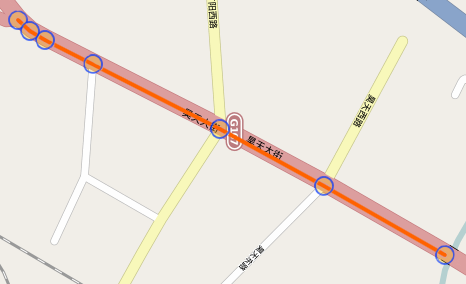
\includegraphics[width=0.8\textwidth]{figures/way-w-nodes.png}
    \caption{A way with nodes}
    \label{fig:waywithnodes}
\end{figure}

\subsection{Generation}
To extract the information in the Osmosis export, so we can use it to model the road network, A XML parser is used. When a node or way tag is read a eqvivalen data structure is created and stored. 
\begin{lstlisting}[style=java, caption=Datastructure for a node]
Node{
	long id;
	double longitude;
	double latitude;
	Ways[] connectedWays;
}
\end{lstlisting}

\begin{lstlisting}[style=java, caption=Datastructure for a way]
Way{
	long id;
	Node[] connectedNodes;
	int type;
}
\end{lstlisting}

We want to model the road network as a graph, but the relation between ways and nodes are not in this format when exported from Osmosis, so we have to work on the data structures generated from the parser.
Besides the original way and node datastructures, we have chosen to create two other classes such that we are able to construct a graph, these are called edges and segments.
Edges are the link between every two nodes and a segment is the link between to intersection nodes. When generating these classes from ways and nodes, we have to check wheter a way has a tag attached to it which describes if the way is oneway or not, because if it is we have to create edges and segments in both directions.

\begin{lstlisting}[style=java, caption=Datastructure for an edge]
Edge{
	long id;
	double length;
	long origin;
	long destination;
	long segment;
}
\end{lstlisting}

\begin{lstlisting}[style=java, caption=Datastructure for a segment]
Segment{
	long id;
	double length;
	long way;
	long origin;
	long destination;
}
\end{lstlisting}

The relation between edges and segments are that each edge of a segment contains a reference to the segment that it is a part of, the same is true from the relation between ways and segments.